%Introduction
\chapter{Introduction}
According to the U.S. Department of Energy \cite{DOE2010} heating and air conditioning energy accounts for approximately 35 - 45\% of the total expenditure within a building.  With such a large investment of energy being used to regulate the temperature of a building, any possible areas of improvement in this area are heavily sought after.  One idea for saving energy is to only regulate the temperature in rooms that are actually in use.  While the problem of determining what rooms are in use can be solved easily by a motion sensor, this problem becomes more difficult when the time to air condition a room is considered along with any considerations related to the exchange of heat between multiple rooms.  If accurate predictive models could be made for the occupancy of any section of the building, then a control scheme may be created that could save on total energy cost.

As another example where the prediction of occupancy may be used to produce significant improvements, consider the United States road ways.  Optimal timing of traffic lights on major road ways across the United States could account for approximately a 22\% reduction in emissions along with a 10\% reduction in fuel consumption \cite{DOT2007}.  As of 2005 the total estimated fuel savings would amount to approximately 17 billions gallons of motor fuels annually.  If accurate estimates of future traffic patterns at each traffic light were available then dynamically changing the light timings to account for such traffic would improve overall traffic flow.

In both of the above scenarios motion through the environment can be captured through a network of many ultra low resolution sensors \cite{Wren2006a} which is defined here to be a sensor with the capacity to sense one bit of data per second.  In the case of buildings, these sensors can take the form of infrared motion sensors, basic camera movement captures and break beam sensors.  For traffic systems the sensors are primarily in road inductive loops.  Utilizing these ultra low resolution sensors to predict future sensor readings will be the focus of this work.

%Problem Statement
\section{Problem Statement}

An explicit assumption to this work is that the sensed observations come from a network of sensors whose readings are spatially and temporally correlated and come from a repeatably predictable environment.  Informally the repeatable environment means that similar observations will happen on a schedule.  Examples of such environments, which have been alluded to in the previous section, are vehicular traffic data and human motion within a building.  

%Given such an environment this work attempts to predict the future expected value of any given sensor within the network for the next $\delta$ %seconds.  This network is assumed to have $N$ sensors and the total number of past readings is $M$ seconds.  A reading from this network is %represented by $x^{(i)}_j$ where $j$ represents the sensor number and $i$ the time.  More generally, $x_{j}^{(i)}$ is used to represent any %time series of length $M$ with $N$ features.  Occasionally it is necessary to index a subset of the time or feature portion of the time series.  %This will be notated using Matlab convention.  Indexing all readings from $i$ to $i + \delta$ will look like $x^{(i:i+\delta)}$.

The goal of this work is to create a hypothesis function $H(x, \delta)$ to predict the value of a sensor $\delta$ seconds in the future.  We will use root mean square (RMS) and mean absolute percentage error (MAPE) as cost functions to minimize.

%The predicted hypothesis function is represented by $H(x, \delta; \theta)$.  Here all values after the semi-colon are parameters of the function.  In the case of the hypothesis function $\theta$ represents a vector of possible weights to be used for the function.

%For the final cost function, we use the common root mean square.  To make the notation of root mean square simpler first we define historic average:

%\begin{equation}
%\label{eq:average}
%A_{historic}(x, i, \delta) = \frac{1}{\delta}\sum_{t = i - \delta}^{i} x^{(t)}
%\end{equation}

%This average holds for $i > \delta$.

%Using historic average, the root mean square cost function is:

%Work on this equation
%\begin{equation}
%\label{eq:rms}
%J_{rms}(x, \delta) = \sqrt{\frac{\sum_{i = \delta + 1}^{M} (A(x, i, \delta) - H(x, i, \delta;\theta))^2}{M - \delta }}
%\end{equation}

%The goal this work is one of discovering the optimal function $H$ and parameterization $\theta$ such that our cost function $J_{rms}$ is minimized.


\section{Approach}

\begin{wrapfigure}{r}{5cm}
\begin{center}
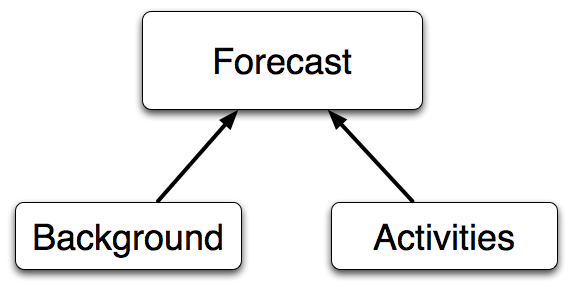
\includegraphics[width=0.30\textwidth]{flow_chart.png}
\end{center}
\caption{Prediction is based on activities and a background model}
\label{fig:flow_chart}
\end{wrapfigure}

Work in the past has attempted to solve this problem with parametric approaches such as fitting an auto regression moving average model (ARMA).  These models use a local history, or in some cases a combination of local and long term history to predict future values.  The primary problem with these approaches is that when training they tend to smooth or ignore deviations from similar time series.

It is our belief that sensed observations within the environments of interest are generated from a combination of a discrete activities along with background motion.  Because activities can overlap or occur at different times with varying amount of background noise present, it is a difficult task for one parametric model to accurately encapsulate all possible combinations of activities.  This is why deviations from such parametric models are typically ignored when training.

We propose modeling these activities using state of the art activity recognition techniques.  Then prediction will be performed using an ensemble predictor taking predictions from all trained activity models and a background model.  

%Approach
\section{Example Activity}

%\begin{figure}[t]
%\begin{center}
%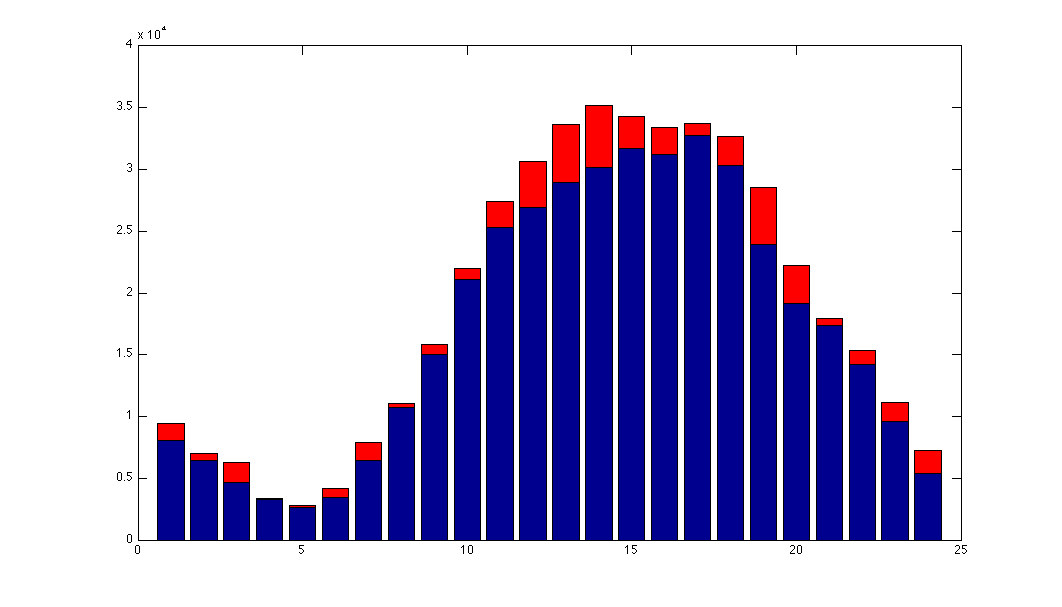
\includegraphics[width=0.8\textwidth]{broncos_max_min.png}
%\end{center}
%\caption{Minimum and maximum count of total Denver traffic for each hour of the day on non-Bronco game Sundays in September and October}
%\label{fig:broncos_max_min}
%\end{figure}

\begin{figure}[ht]
\begin{center}
\subfloat[][Away games Sunday] {
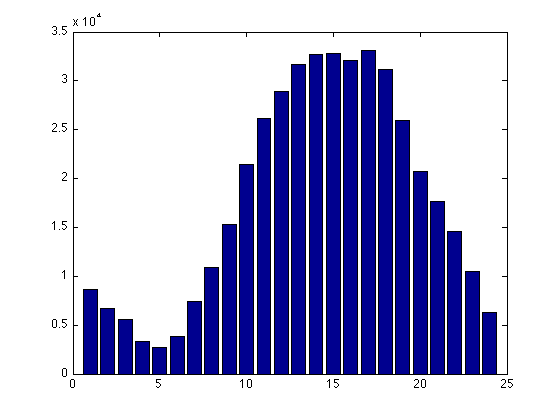
\includegraphics[width=0.45\textwidth]{broncos_off4.png}
\label{fig:broncos_off}
}
\subfloat[][Broncos game Sunday] {
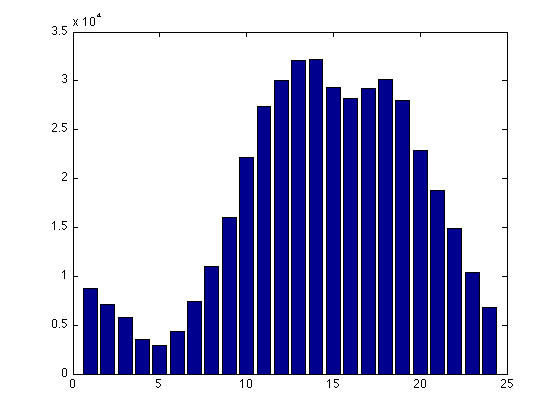
\includegraphics[width=0.45\textwidth]{broncos4.png}
\label{fig:broncos_on}
}
\end{center}
\caption{Total number of cars passing major highway sensors on Sundays in September and October 2010}
\label{fig:broncos}
\end{figure}

Due to the assumption of repeatability in our sensed environment, developing a model that captures repeated behavior accurately is important.  To show an example of this refer to figure~\ref{fig:broncos_max_min}.  This figure shows total traffic flow from ten freeway and road sensors located around downtown Denver.  The horizontal axis represents time of day given in hours.  The vertical axis is total counts.  The data collected for this figure is from non broncos game Sundays during September and October.  The blue bar represents the lowest total value across all Sundays for that hour of the day.  The red bars represent the maximum value.  

This figure shows how little variation there is in traffic patterns.   Time of day alone tends to be a good predictor \cite{kwon2000} when used for general historic trends, yet it is infrequently used when predicting traffic patterns.  

Prediction from a time of day model is represented by:

\begin{equation}
\label{eq:time_of_day}
H_{TOD}(x,\delta) = H_{TOD}(M, \delta)
\end{equation}

This form of model does not depend on a time series of input data, instead it only needs $M + \delta$ which is the time to predict.  One problem with time of day prediction is that it does not account for local variations in time or space.  Handling such variations will be the emphasis of activity models.

Recognition and modeling of localized variations from the time of day model are necessary to improve the predictive capabilities of the time of day model.  Such variations are defined in this work as activities.  

An example of such an activity would be the effect of Broncos games on the traffic of downtown Denver.  Figure~\ref{fig:broncos} shows the total counts of Denver traffic for each hour of the day averaged for the first four Sunday Broncos Home games and for the first four Sunday away games.  Comparing figure~\ref{fig:broncos_off} with figure~\ref{fig:broncos_on} it is evident that a noticeable change in traffic patterns occur from approximately noon until approximately 2:00 pm.  This traffic change corresponds with a 2:05pm kickoff time for the game.  

Typical non game day Sundays are repetitive and follow a predictable traffic pattern.  Similarly typical game day Sundays are repetitive and follow a predictable traffic pattern around the time of the game.  A well implemented prediction system must either include knowledge of Broncos game times or be able to dynamically realize the presence of a Broncos game and handle prediction accordingly.  Due to the difficulty of modeling all scheduled activities with a time of day model, we propose using activity models to improve predictive accuracy.

An activity is defined as a time series of features which allow for the prediction of some time in the future.  Unlike a time of day model, activities use historic data and a subset of features to predict some time $M + \delta$ in the future.

\begin{equation}
\label{eq:activity_predict}
H_{activity}(x, \delta) = H_{activity}(x^{(i:M)}, \delta)
\end{equation}

\begin{figure}[t]
\begin{center}
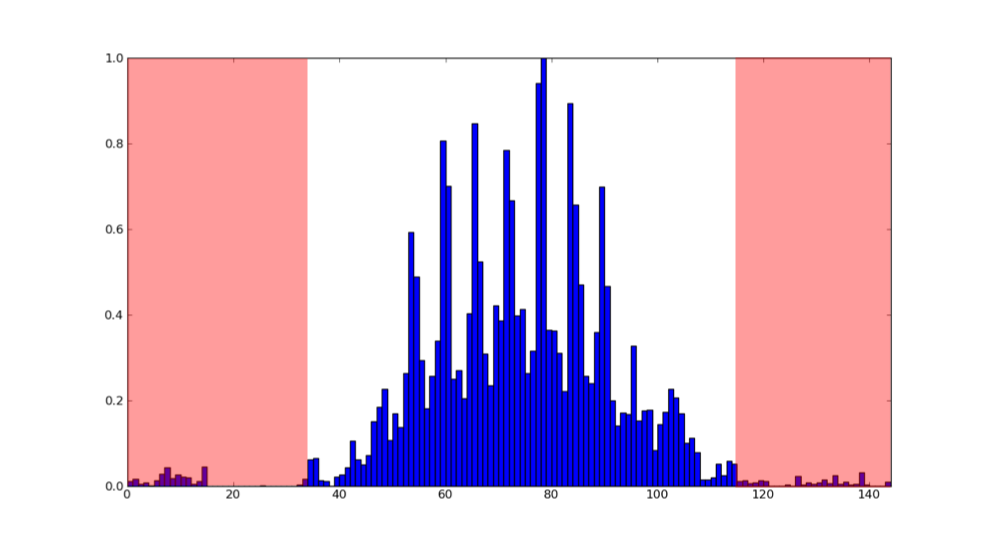
\includegraphics[width=0.8\textwidth]{low_traffic.png}
\end{center}
\caption{Total motion counts for a day within a college classroom building}
\label{fig:low_traffic}
\end{figure}

One drawback to prediction is when the same activity leads to different future activities.  Figure~\ref{fig:low_traffic} shows one example of this problem.  This figure displays a normalized graph of people counts within the Colorado School of Mines Brown Building for one day using 10 minute windows.  Not surprisingly there is relatively low activity throughout the building during the early morning and late night.

Using activity modeling alone to predict motion within this building leads to areas of lengthy inactivity corresponding to an activity.  Due to computational and complexity constraints on the length of time series used to train activities it is expected that activities will correspond to relatively short periods of time.  The classification of early morning time windows from the Brown Building data will look like a long string of the same low traffic activity $\{..., a_{low}, a_{low}, a_{low}, ...\}$.   Thus $a_{low}$ typically follows $a_{low}$, but what happens in the morning when people start to enter the building?  There will be an instance where $a_{low}$ is followed by a different activity.  Similarly, if $a_{low}$ happens during the middle of the day it will be followed by a different activity.  For a given activity It is not the case that the same activity follows it irrespective of time.  

\section{Contributions}  
In general activity modeling work has focused more on the capability to recognize different activities.  This work is instead focused on activity prediction capabilities.  In a later section we introduce a measure how soon a recognized activity can be used for prediction.

Also, other work in the area of traffic prediction tends to use models that are based on a short history of readings.  Such work has problems predicting activities which occur with varying amount of background noise (i.e. Prediction would be poor if the Broncos had an evening game instead of an afternoon game).  Typically all data is modeled together and no distinction is made between background (time of day) data and activity data.  This work is different due to the use of activity modeling techniques to account for predictable variations in the time of day model.  

There has also been a lack of research into discovery of the optimal timeframe and spatial influence of other sensors when considering activities.  Other predictive approaches tend to use the entire network.  We instead search for the best spatial features and temporal scales to perform prediction on.


\section{Structure of the Proposal}
The remainder of this proposal first outlines current work related to traffic prediction and activity modeling and recognition in section two.  Section three gives a summary of each dataset used in this work.  Section four details specific pieces of the overall approach.  All of the approach is not solved and where possible this section details potential ways to proceed with each unsolved part of the approach.  Finally section five is a time line of when the remaining work is expected to be completed.

